\documentclass{article}
\usepackage{xcolor}
\usepackage[preprint]{corl_2026}
\usepackage{booktabs}
\usepackage{graphicx}
\graphicspath{{figures/}}
\usepackage{amsmath}
\usepackage{xspace}
\usepackage{url}

\newcommand{\pizero}{$\pi_0$\xspace}
\newcommand{\pizerofive}{$\pi_{0.5}$\xspace}
\title{Higher Success, New Failures:\\Measuring Per-State Regressions in VLA Policy Updates}
\author{Qiang Guo\\Independent Researcher\\\texttt{glay.guo@foxmail.com}}
\hypersetup{
  pdftitle={Higher Success, New Failures: Measuring Per-State Regressions in VLA Policy Updates},
  pdfauthor={Qiang Guo},
  pdfsubject={Research preprint; expanded manuscript, October 2026},
  pdfkeywords={Vision-language-action models, paired evaluation, regression testing, LIBERO}
}

\begin{document}
\raggedbottom
\maketitle

\begin{abstract}
Quantized, distilled or otherwise accelerated vision-language-action (VLA) policies are judged by
the change in their aggregate success rate. A deployment also needs to know whether the new policy
fails where the old one succeeded. Comparing the two policies with one rollout per initial state
cannot distinguish an update effect from rollout variability: in VLAQuantBench's public LIBERO
records, rerunning an unchanged configuration with a new seed changes the outcome of up to a
quarter of the initial states. We define a state as a LIBERO initial state together with its scene
seed, repeat each state under both policies with shared policy-seed plans, and use exact paired
tests with false-discovery control. On X-VLA in LIBERO-10, the first-rollout old-versus-old floor
is 2--3 flips per 100 states. Three-bit weight rounding concentrates a 20-point aggregate drop
on a few tasks; seven states change from 5/5 to 0/5 successes, but the five-repeat screen is
underpowered after multiplicity correction. Four-bit rounding and fewer denoising steps produce
no detected statewise regression, which does not certify their absence. BF16 leaves the
aggregate nearly flat but identifies one candidate state; 20 fresh paired rollouts confirm its
loss (18/20 against 4/20, exact $p=2.59\times10^{-4}$). This is evidence about one independently
retested state, rather than an estimate of regression prevalence or a physical safety certificate.
\end{abstract}
\keywords{Vision-language-action models, quantization, evaluation, regression testing}

\section{Introduction}
VLA updates change precision, inference steps or checkpoints. Aggregate success
rates~\citep{xu2026vlaquantbench} do not answer an operator's question: where does the new
policy fail when the validated old one succeeded? The question resembles backward compatibility
in classification~\citep{bansal2019updates,srivastava2020compat,yan2021pcr}, where a more accurate
model can still err on inputs the old one got right. Closed-loop control adds rollout randomness
and evolving observations, which complicate the interpretation of an individual outcome change.

On LIBERO~\citep{liu2023libero}, \citet{sawada2026paired} find substantial outcome changes under
compound perturbations; \citet{yardimci2026collapse} report task collapse under online RL.
An observed old-success/new-failure pair may be an update-induced loss, a stochastic fluctuation,
or a change in the scene. These explanations require different responses. A single rollout does
not distinguish them, even when aggregate success rises.

Our contributions are an empirical noise baseline from four models and four suites
(Section~\ref{sec:floor}), a paired statewise protocol with repeat controls
(Section~\ref{sec:method}), and one fresh confirmation of a BF16 loss in
X-VLA~\citep{zheng2025xvla} (Section~\ref{sec:xvla}). We distinguish single-rollout
flips, repeated-state candidates and fresh confirmation, using established
statistical tools rather than proposing a new test.

\begin{figure}[t]
  \centering
  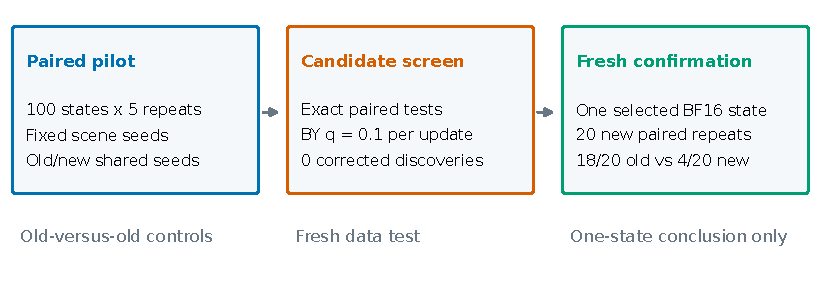
\includegraphics[width=\linewidth]{paired-protocol.pdf}
  \caption{Discovery and confirmation use different outcomes. The 100-state pilot yields
  descriptive candidates but no BY-corrected discoveries. One selected BF16 candidate is
  tested on 20 fresh pairs, excluding its pilot outcomes. Old-versus-old controls accompany
  the pilot; confirmation supports a conclusion about the selected state only.}
  \label{fig:protocol}
\end{figure}

\section{Paired statewise evaluation}
\label{sec:method}
\paragraph{State identity.}
LIBERO provides an initial-state file per task for the robot and movable objects. Fixtures
such as cabinets and stoves can nevertheless change when a scene is rebuilt: three hard
resets of LIBERO-10 task 0, state 0 gave three cabinet positions. We define a state
$s=(\text{task},\text{initial-state index},\text{scene seed})$ and use a fixed scene-seed plan
for comparisons of policy variants. This identity is an operational evaluation definition,
not proof that every hidden simulator variable is identical.

\paragraph{Pairing.}
Each state is rolled out $n$ times per variant. The policy-noise seed plan depends on the
task, batch and base seed, and does not depend on the variant. We pair outcomes by state and
repeat index and check that their recorded policy seeds match. Shared seeds can reduce
comparison noise, but do not guarantee identical noise consumption or trajectory coupling
after the policies diverge. Each historical evaluation batch creates a new vector environment.
The archived records do not contain full reset-state or camera digests
(Appendix~\ref{app:reproducibility}).

\paragraph{Exact paired test.}
For state $s$, let $b_s$ count old-success/new-failure pairs and $c_s$ count
old-failure/new-success pairs. We test the one-sided null that harmful discordance is
no more likely than beneficial discordance. At the null boundary, conditional on
$b_s+c_s$ discordant repeats,
\begin{equation}
 p_s=\sum_{k=b_s}^{b_s+c_s}{b_s+c_s\choose k}2^{-(b_s+c_s)}.
 \label{eq:paired}
\end{equation}
Set $p_s=1$ when there is no discordance. This is the conditional exact paired
McNemar/binomial test, rather than an unpaired comparison of success counts.
Validity assumes independent paired repeats from a stable evaluation process; dependence
within each old/new pair is allowed. Pseudorandom seed matching alone does not establish
these assumptions.

\paragraph{Multiplicity and descriptive summaries.}
For each update, we apply Benjamini--Yekutieli (BY)~\citep{benjamini2001dependency}
at FDR $q=0.1$ across its 100 statewise regression hypotheses. BY permits arbitrary
dependence between valid statewise $p$-values. Improvement tests, where reported, form a
separate directional family; neither directional result constitutes a joint guarantee
over both directions or over all searched updates.

We also report the Jeffreys posterior
$\Pr\{\mathrm{Beta}(b_s+1/2,c_s+1/2)>1/2\}$ for the direction of discordance.
This posterior is a descriptive candidate score: it is not a multiplicity-adjusted
discovery rule or a posterior on the magnitude of the success loss.
Aggregate intervals resample the 100 observed states 4,000 times with a fixed analysis
seed and use the 2.5th and 97.5th percentiles of their mean paired differences.
They are descriptive state-bootstrap intervals, conditional on this inventory and its
observed repeats, rather than a guarantee for unseen tasks or states.
The \emph{naive} flip count uses repeat 0 only.

\paragraph{Old-versus-old controls.}
We compare a policy with itself using new policy seeds, pairing planned repeat indices.
A separate control changes scene seeds and pairs task/initial-state indices. That control
is a scene perturbation, not an identical-state policy update. Both measure repeat
variability; they do not establish that an individual update-induced loss is absent.

\paragraph{Why discovery needs a second stage.}
With $n=5$, the smallest attainable one-sided exact $p$-value is $2^{-5}=1/32$,
even if every pair is harmful. For 100 states, the BY rank-1 cutoff is
$q/(100H_{100})\approx1.93\times10^{-4}$, with
$H_{100}=\sum_{i=1}^{100}1/i$. Even the rank-100 cutoff,
$q/H_{100}\approx0.0193$, is below $1/32$. Thus no state can pass this pilot's
BY rule, regardless of its outcome pattern. This is a limitation of the design,
not evidence that the updates preserve every state.
Figure~\ref{fig:resolution} shows the attainable resolution. Thirteen entirely harmful
pairs would cross the rank-1 cutoff, but this best-case calculation is not a general
sample-size or power recommendation.

\begin{figure}[t]
  \centering
  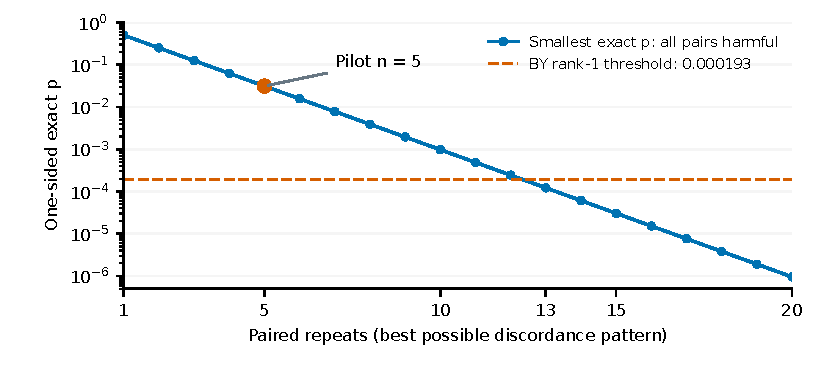
\includegraphics[width=\linewidth]{test-resolution.pdf}
  \caption{Best-case test resolution. The blue curve assumes every repeat is a harmful
  discordance; any gain or concordance raises the attainable $p$-value for a fixed total
  number of repeats. The orange line is the BY rank-1 cutoff for 100 hypotheses at $q=0.1$.
  The pilot cannot produce a corrected discovery. The crossing at 13 repeats is an
  arithmetic bound under this extreme outcome pattern, not a power analysis.}
  \label{fig:resolution}
\end{figure}

\section{How noisy is one rollout per state?}
\label{sec:floor}
VLAQuantBench~\citep{xu2026vlaquantbench} released episode records from its 409 closed-loop
runs under an MIT licence. Its LIBERO configurations cover four models and four suites.
Each configuration uses 200 states (20 initial states for each of 10 tasks), except
X-VLA, which uses 190. Twenty configurations are repeated with additional seeds.
We reanalyze release commit \texttt{4a2cb7c}; these are public benchmark outcomes,
separate from our X-VLA experiments.

\paragraph{Unchanged configurations flip many states.}
Table~\ref{tab:floor} and Figure~\ref{fig:floor} show outcome changes between seeds
of the same configuration. Near the ceiling, the count is small
(1--8 of 200 at 97.5--99.5\% success), but rises as success falls:
21--32 states at 72--88\% and 32--50 at 60--71\%.
The plot includes all released baseline-versus-update comparisons and all 20 repeated
configurations; representative rows appear in the table.

\paragraph{Equal seed labels do not establish pairing.}
Different configurations run with the same seed disagree on as many states as with
different seeds. For example, \pizerofive baseline against its W4A4 action-head variant
on LIBERO-Object differs at 77.3 states with matching seed labels and 78.0 across seeds
(means over the available comparisons). The released labels do not by themselves
demonstrate episode-level common-random-number coupling. We use reruns to contextualize
the observed flips, without assigning the public cross-configuration flips an exact
paired significance interpretation.

\paragraph{State difficulty is heterogeneous.}
For \pizerofive with a W4A4 action head on LIBERO-Object (61\% success), 43 states fail
under all three seeds and 85 succeed under all three. If every state instead had the
same success probability, independence would predict approximately 12 and 46.
This contrast supports heterogeneity in state difficulty; it does not identify a
causal update loss from one rollout.

\paragraph{Consequence for a small aggregate change.}
For \pizero~\citep{black2024pi0} on LIBERO-10 with W8 weights, aggregate success moves
from 48.5\% to 47.5\%, while 24 states flip to failure and 22 to success.
A seed change alone produces a comparable flip count at that success level.
Interpreting the locations of those update flips requires repeated outcomes.

\begin{table}[t]
  \centering
  \small
  \caption{Representative unchanged-configuration reruns in VLAQuantBench (200 states).
  Success rates and flips are raw descriptive counts. ``Never/always/mixed'' partitions
  states across all listed seeds. The reanalysis records contain all 20 repeated configurations.}
  \label{tab:floor}
  \setlength{\tabcolsep}{3pt}
  \begin{tabular}{llccc}
    \toprule
    Suite/model & Configuration & Success by seed & Pair flips & Never/always/mixed\\
    \midrule
    Object/\pizerofive & baseline & .990 .985 .995 & 5, 1, 4 & 0/195/5\\
    Object/\pizerofive & W4A4, action head & .600 .630 .610 & 44, 50, 50 & 43/85/72\\
    Spatial/\pizerofive & W4A4, action head & .705 .705 .685 & 44, 36, 32 & 34/110/56\\
    Spatial/\pizerofive & W4A4, MLP only & .880 .875 & 29 & 10/161/29\\
    10/OpenVLA-OFT & W3, no fc2 in head & .935 .915 .910 & 8, 7, 9 & 11/177/12\\
    \bottomrule
  \end{tabular}
\end{table}

\begin{figure}[t]
  \centering
  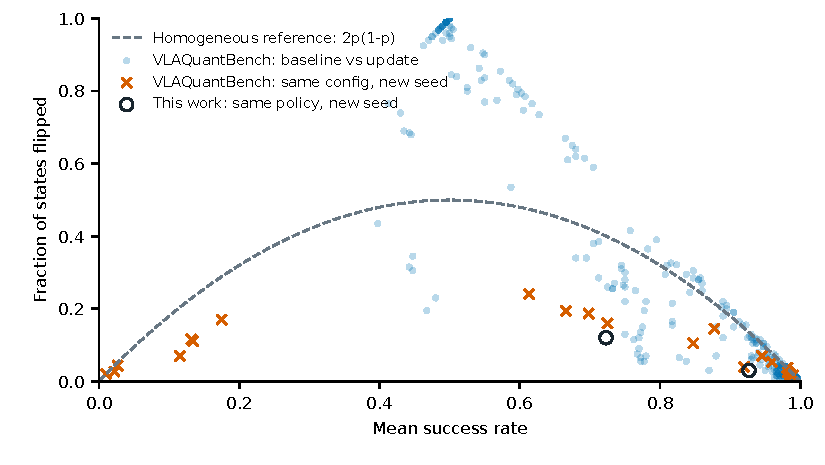
\includegraphics[width=\linewidth]{noise-floor.pdf}
  \caption{Outcome flips versus mean success. Blue dots: public baseline-versus-update
  comparisons. Orange crosses: unchanged public configurations with new seeds (mean
  over available seed pairs). Open circles: our FP32 and W3 policy-seed controls,
  first repeat only. The dashed homogeneous-state reference $2p(1-p)$ assumes two
  independent rollouts with common success probability $p$; it is not a fitted noise
  model or a confidence bound.}
  \label{fig:floor}
\end{figure}

\section{X-VLA precision and inference-step updates}
\label{sec:xvla}
\paragraph{Setup.}
We evaluate \texttt{lerobot/xvla-libero} using LeRobot 0.6.1~\citep{cadene2026lerobot} on LIBERO-10:
10 tasks $\times$ 10 initial states $\times$ 5 repeats, absolute end-effector control,
10 flow-matching steps, and a 520-step limit. Every failure in the FP32 run is a timeout.
Our baseline succeeds in 92.6\% of episodes; VLAQuantBench uses a 900-step horizon and
reports 97.9\% for the same model identifier. These protocols differ, so their rates
are context rather than a controlled replication.

The W3 and W4 variants round all 267 linear layers (792M parameters) to a symmetric
integer grid with one scale per group of 128 inputs, then store the weights dequantized.
They measure a numerical weight perturbation, not the speed or memory efficiency of
an integer inference kernel. The two-step variant changes the flow-matching step
count; BF16 changes model numerical precision.

\begin{table}[t]
  \centering
  \small
  \caption{FP32 versus each variant: 100 states, 5 repeats per state.
  $\Delta$ and descriptive 95\% state-bootstrap intervals are in percentage points.
  Naive flips use repeat 0 (harm/gain). BY counts use separate regression/improvement
  families at $q=0.1$. Posterior counts are descriptive. FP32 baseline success is .926.}
  \label{tab:xvla}
  \setlength{\tabcolsep}{3.5pt}
  \begin{tabular}{lccccc}
    \toprule
    Variant & Success & $\Delta$ [95\% CI] & Naive & BY & $P(\text{worse})>0.9$\\
    \midrule
    FP32, new policy seeds & .928 & $+0.2$ [$-1.0$, $+1.4$] & 0/3 & 0/0 & 0\\
    FP32, new scene seeds & .930 & $+0.4$ [$-0.4$, $+1.2$] & 0/2 & 0/0 & 0\\
    W4, group 128 & .918 & $-0.8$ [$-3.2$, $+1.2$] & 4/2 & 0/0 & 1\\
    W3, group 128 & .726 & $-20.0$ [$-26.8$, $-13.4$] & 23/2 & 0/0 & 26\\
    2 flow steps (of 10) & .932 & $+0.6$ [$-0.6$, $+2.0$] & 1/3 & 0/0 & 0\\
    BF16 & .916 & $-1.0$ [$-4.6$, $+2.2$] & 4/3 & 0/0 & 5\\
    \bottomrule
  \end{tabular}
\end{table}

\paragraph{The floor is low for high-success fixed states.}
FP32 against itself changes 13 of 500 outcomes under new policy seeds and 8 under
new scene seeds. No state's success count changes by more than two. Of the 100 states,
88 succeed in all five FP32 repeats and five fail in all five.
At this success level and under this protocol, reruns are close to replay.
The scene-seed control does not show a larger flip count than the policy-seed control,
but this small comparison does not establish that fixture placement is irrelevant.
At lower success, W3 against itself changes 73 of 500 outcomes. Its first repeats give
3 harmful and 9 beneficial flips; four states have posterior direction probability
above 0.9, and none passes BY.

\paragraph{W4: descriptive candidates, no corrected discovery.}
Its six naive flips are twice the first-repeat policy-seed floor. The most affected
state changes from 5/5 to 1/5 (paired $p=0.0625$). No state passes correction,
as expected from the screen's resolution limit. This is not evidence of equivalence
or preservation at every state.

\begin{figure}[t]
  \centering
  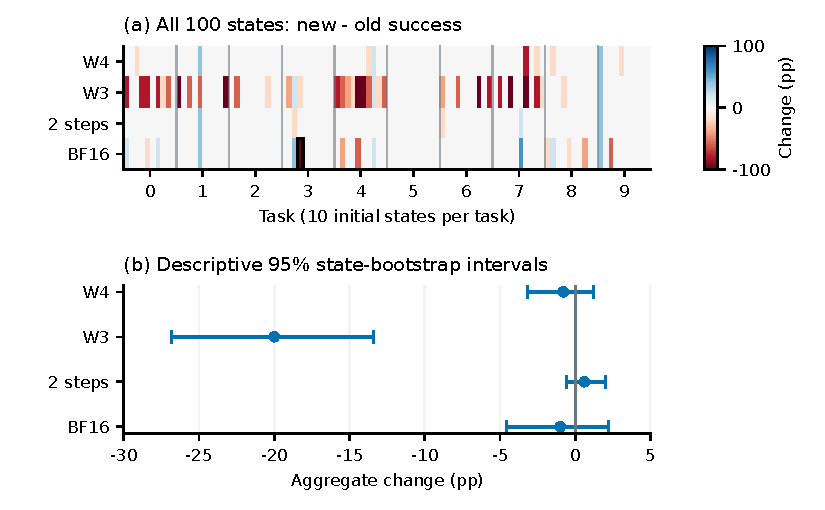
\includegraphics[width=\linewidth]{statewise-pilot.pdf}
  \caption{All 100 pilot states in fixed task/initial-state order.
  (a) Empirical success differences in percentage points, with all five repeats.
  Black outline: task 3, initial state 3, selected for BF16 follow-up (indices start at zero).
  (b) Aggregate differences and descriptive state-bootstrap intervals.
  These locations are candidate patterns: every update has zero BY-corrected
  discoveries at five repeats.}
  \label{fig:states}
\end{figure}

\paragraph{W3: large losses concentrated in particular states.}
The aggregate drop is 20 points, but its location is uneven. Tasks 5, 8 and 9 retain
96--100\% success, while tasks 0, 4 and 7 lose 40--52 points. Seven states change from
5/5 to 0/5. None passes correction; 26 have posterior direction probability above 0.9,
compared with four in the W3 rerun control.
The first-repeat protocol reports 23 harmful and two beneficial flips.
Every W3 failure times out. Its successful episodes average 265 steps, compared with
256 for FP32. VLAQuantBench's W3 variant loses only 3.2 points under its quantizer and
900-step horizon. Quantizer and horizon differ together, so the source of that
between-protocol difference cannot be isolated here.

\paragraph{Two flow steps: higher success with one naive new failure.}
Reducing the flow-matching head from 10 to two steps changes success from 92.6\%
to 93.2\%. The first repeat still shows one new failure; that state changes from 5/5
to 4/5. This is compatible with the observed repeat floor and is not a corrected
statewise discovery. The descriptive aggregate interval also includes zero.

\paragraph{BF16: one candidate confirmed with fresh pairs.}
BF16 changes the aggregate by $-1.0$ points, with a descriptive interval including zero.
Recorded episode lengths differ in 422 of 500 pairs; these logs do not provide a full
trajectory-distance measure. One state changes from 5/5 to 0/5
(uncorrected paired $p=0.03125$). The pilot alone does not establish its regression.

We selected this state (task 3, initial state 3) for a targeted follow-up with 20 fresh
pairs and a new policy-seed plan. The pilot outcomes are excluded from the test.
FP32 succeeds in 18/20 and BF16 in 4/20. The paired table contains three joint
successes, 15 harmful discordances, one beneficial discordance and one joint timeout
(Figure~\ref{fig:confirmation}). The one-sided exact probability is
\begin{equation}
 p=\Pr\{\mathrm{Binomial}(16,1/2)\ge15\}
   =\frac{{16\choose15}+{16\choose16}}{2^{16}}
   =0.0002593994.
\end{equation}
The single fresh follow-up provides evidence of a loss at this selected state,
conditional on the paired-test assumptions and the evaluation protocol. All 16 BF16
failures are timeouts. It does not estimate how common such losses are across the
100 states, other updates, different horizons or physical robots.

\begin{figure}[t]
  \centering
  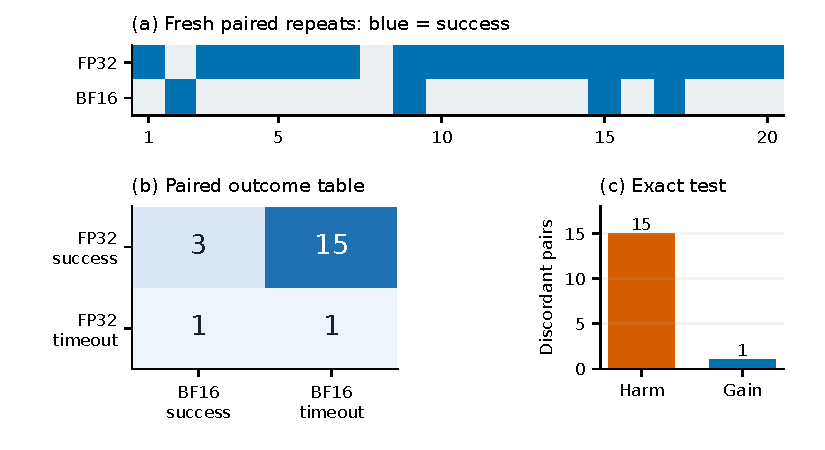
\includegraphics[width=\linewidth]{fresh-confirmation.pdf}
  \caption{Fresh BF16 confirmation at one selected state. (a) All 20 paired binary
  outcomes in repeat order; light grey denotes timeout. (b) The full paired table.
  (c) Fifteen harmful versus one beneficial discordance yield exact one-sided
  $p=0.0002593994$. The state was selected from the pilot, but only new outcomes
  enter this single confirmation test.}
  \label{fig:confirmation}
\end{figure}

\section{Related work and scope}
Backward compatibility~\citep{bansal2019updates,srivastava2020compat,yan2021pcr}
motivates reporting new errors even when total accuracy improves. In a closed-loop VLA,
outcomes depend on action sampling and the evolving environment; therefore a binary
flip needs repeat controls before it can be interpreted as a persistent local loss.
VLAQuantBench~\citep{xu2026vlaquantbench} measures post-training quantization across
models and suites. We reuse its released records to measure repeat variability and
add a repeated-state X-VLA study with independent candidate confirmation.

Compound robustness evaluation~\citep{sawada2026paired} tests perturbation sensitivity;
online-RL task collapse~\citep{yardimci2026collapse} concerns changes during adaptation.
Deployment comparisons~\citep{islam2026onnx} and update-admission
audits~\citep{ma2026admission} examine aggregate behavior or synthetic acceptance
settings. Our endpoint is the location of a precision or inference-step update's
candidate loss in a real closed-loop simulation benchmark.
Sequential policy comparison~\citep{snyder2025step} suggests allocating additional
rollouts to uncertain comparisons. We do not claim a new sequential stopping rule,
nor reuse fixed-sample $p$-values after unrestricted outcome-dependent stopping.

\section{Discussion and limitations}
Report paired outcomes and old-versus-old controls alongside aggregate success,
distinguishing \emph{candidate}, \emph{confirmed loss}, and \emph{not resolved}.
The five-repeat screen is incapable of rejecting any statewise hypothesis under
its BY rule; a small aggregate change does not overcome that limit.

The new experiments use one model in simulation, a limited fixed inventory and
a 520-step timeout criterion. They do not measure physical hazard, unseen-scene
robustness, hardware latency or integer-kernel performance. Public-data reanalysis
broadens the noise observations, but does not make our precision experiment
a multi-model study.

Exact tests require stable independent paired repeats. BY permits dependence across
valid state tests; it cannot repair invalid within-state sampling, systematic
reset differences or corrupted outcomes. Historical records omit some provenance
needed for a fully audited replay. The BF16 follow-up measures a numerical update
under this protocol without identifying its internal failure mechanism.

A prospective study should freeze state inventories and update families, validate
reset equality, record immutable model/simulator identities, and budget multiplicity
and confirmation before collection. Retain timeouts, infrastructure failures and
uncertain decisions. These are future improvements, not assertions that unrecorded
historical checks were performed.

\clearpage
\bibliography{references}
\clearpage
\appendix
\section{Reproducibility and evidence boundaries}
\label{app:reproducibility}
\paragraph{Archived outcomes.}
The archived research files contain the public-data reanalysis,
eight 500-episode pilot/control files, and two 20-episode follow-up files.
Rows record task, initial-state index, scene seed, repeat index, policy seed,
success, steps, model family, variant and suite. The analysis rejects duplicate
repeat identities, unequal state inventories and undeclared policy-seed mismatches.
The figure builder checks paired identities, rederives all plotted differences,
confirms the follow-up seed separation, and records SHA-256 identities of its inputs.
These hashes identify the archived files; they do not prove that missing historical
metadata was captured at collection time.

\paragraph{Numerical reanalysis.}
For a same-scene update, paired rows match
$(\text{task},\text{initial state},\text{scene seed},\text{repeat})$.
For the policy-seed control, differing policy seeds are explicitly declared.
The scene-seed control explicitly drops the scene seed from matching and therefore
answers a different question. The bootstrap uses analysis seed 1 and 4,000 state
resamples. The analysis implementation includes boundary checks for discordance
tests, BY correction and pairing failures.

\paragraph{Historical seed plan.}
Scene seeds use the declared base, task and initial-state index. Policy random seeds
depend on the base, task and batch. The FP32 pilot uses base seed 1000; its
independent-policy-seed control uses 2000. The targeted follow-up uses base 3000.
Torch TF32 is disabled and deterministic settings are requested with warnings
rather than guaranteed deterministic execution. New vector environments are created
for each historical batch. Batch composition can affect the consumption of random
numbers; changing it is not a documented equivalent replay.

\paragraph{Provenance gaps.}
The historical episode files do not include immutable checkpoint revisions,
complete reset-state/camera digests, or full action and observation streams.
The evaluator loads a model by its repository identifier. A currently cached
revision cannot establish the exact historical download, so no retrospective
checkpoint pin is asserted here. These omissions limit bit-exact reproduction
and any stronger causal claim based on hidden simulator-state equality.
Later prospective reset audits and health checks are separate work and do not
constitute new evidence in this manuscript.

\paragraph{Interpretation checklist.}
The public-data flips estimate observed repeat disagreement; they are not a
statewise significance result. The pilot heatmap and posterior identify candidates;
none is a BY-corrected discovery. The fresh BF16 test confirms one selected
candidate under its assumptions; it is not an estimate of population prevalence.
Non-detection is not equivalence, and simulated weight rounding is not a
hardware acceleration measurement.

\paragraph{Local reproducibility.}
Run \texttt{python3 build\_figures.py} from this revision directory, then
\texttt{make all}. The figure builder reads the repository's archived results.
The arXiv upload archive is a flat allowlist of TeX, bibliography output, the
unmodified third-party style and the five vector figure PDFs. Its clean-room
build does not require the raw data, Python environment or a network connection.
The expanded preprint uses the same research outcomes as the workshop submission;
it adds exposition, figures and explicit evidence limitations.

\end{document}
